\begin{document}
Pel que fa a l'anàlisis de costos, s'ha intentat segregar segons els diferents paràmetres on el sistema es pot derivar, que són:
\begin{itemize}
	\item La mida del sistema agregat, és a dir, el nombre de comptadors d'un barri.
	\item L'algorisme emprat per tal de realitzar el logaritme discret.
\end{itemize}
No obstant això, anteriorment s'ha especificat certes propietats que comporta el sistema:
\begin{itemize}
	\item Es considera que entre ronda i ronda hi haurà, com a mínim, un interval de 15 minuts, és a dir, la lectura que es passarà correspondrà al consum dels últims 15 minuts.
	\item Per tal de no sobrecarregar l'algoritme del logaritme discret, les lectures dels comptadors han de tenir un cert grau de control en la seva mida en bits.\\
	 Primer, es va pensar realitzar l'anàlisis amb lectures pseudo-aleatòries. Per aquesta raó, està creada la classe \texttt{RandomConsumption}, que enviava un enter positiu aleatori de, com a màxim, 13 bits. No obstant això, amb la intenció de tenir una simulació més realista, s'ha buscat un \textit{dataset} que ens permeti visualitzar el consum elèctric d'una llar \cite{kaggle-consumption} i crear un lectures més properes a les reals. Les dades trobades aporten el consum elèctric amb una freqüència de mostreig d'un minut durant aproximadament 4 anys en tres espais diferents de la llar, tal i com es pot apreciar a la \textit{Taula \ref{tab:ex-kaggle}}.
	\begin{table}[H]
		\centering
			\begin{tabular}{llrrr}
				\toprule
				{} &           date\_time &  Sub\_metering\_1 &  Sub\_metering\_2 &  Sub\_metering\_3 \\
				\midrule
				0 & 2006-12-16 17:24:00 &             0.0 &             1.0 &            17.0 \\
				1 & 2006-12-16 17:25:00 &             0.0 &             1.0 &            16.0 \\
				2 & 2006-12-16 17:26:00 &             0.0 &             2.0 &            17.0 \\
				3 & 2006-12-16 17:27:00 &             0.0 &             1.0 &            17.0 \\
				4 & 2006-12-16 17:28:00 &             0.0 &             1.0 &            17.0 \\
				...\\
				\bottomrule
			\end{tabular}
		\caption{Primeres files del dataset.}
		\label{tab:ex-kaggle}
	\end{table}
	Primer, s'han tractat les dades agregant els consums dels diferents espais per trobar el consum total de la llar. Seguidament, un cop tenint el consum de la llar agregat, es realitza la mitjana d'aquest valor en funció del temps, és a dir, la mitjana de tots els dies en funció de l'hora i el minut en què s'ha realitzat la lectura. Una part del resultat obtingut es mostra a la \textit{Taula \ref{tab:ex-kaggle-mean}}, com a exemple.
	\begin{table}[H]
		\centering
		\begin{tabular}{lrrr}
			\toprule
			{} & hour & min & consumption mean \\
			\midrule
			0 &    0 &   0 &    4.537868 \\
			1 &    0 &   1 &    4.524544 \\
			2 &    0 &   2 &    4.568022 \\
			3 &    0 &   3 &    4.599579 \\
			4 &    0 &   4 &    4.600281 \\
			5 &    0 &   5 &    4.666199 \\
			6 &    0 &   6 &    4.443198 \\
			7 &    0 &   7 &    4.525947 \\
			8 &    0 &   8 &    4.596073 \\
			...\\
			\bottomrule
		\end{tabular}
	\caption{Primeres files del dataset transformat realitzant la mitjana}
	\label{tab:ex-kaggle-mean}
	\end{table}
	   Així doncs, es pot visualitzar la mitjana trobada pel consum elèctric total de la llar en funció del horari de la següent forma:
\begin{figure}[H]
	\centering
	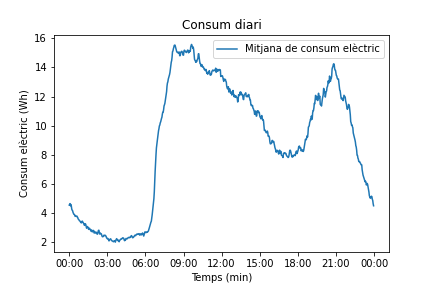
\includegraphics[width=8cm]{imgs/cost/consumptionmin.png}
	\caption{Mitjana de consum diari.}
	\label{fig:consumptionmin1}
\end{figure}
Per tal de variar les lectures entre diferents comptadors, s'ha creat una cota màxima i una cota mínima per establir un rang de possibilitats:
\begin{figure}[H]
	\centering
	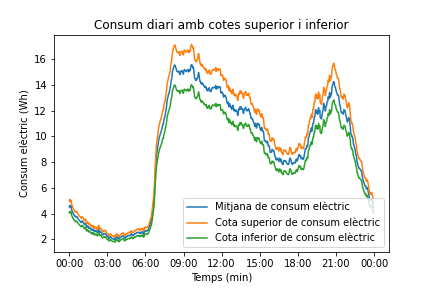
\includegraphics[width=8cm]{imgs/cost/consumptionmin2.png}
	\caption{Mitjana de consum diari amb cotes superior i inferior.}
	\label{fig:consumptionmin2}
\end{figure}
Finalment,  s'han agregat els consums de 15 en 15, ja que la lectura es passarà en intervals de 15 minuts, com ja s'ha mencionat anteriorment. D'aquesta manera, cada quart d'hora correspon a una classe d'equivalència. \\
En conclusió, es pot afirmar que agafant un nombre pseudo-aleatori dins del rang possible corresponent a cada ronda, es pot acabar generant un dia de lectures més o menys fidel a la realitat. No obstant això, cal esmentar que s'ha modificat lleugerament la cota superior per tal de crear més variació entre comptadors, tal i com es pot veure a la \textit{Figura \ref{fig:consumption2}}.
\begin{figure}[H]
	\centering
	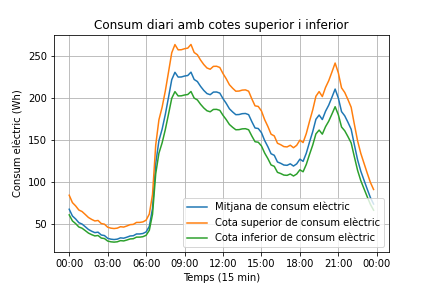
\includegraphics[width=8cm]{imgs/cost/consumption2.png}
	\caption{Gràfica de lectures amb cotes superior i inferior.}
	\label{fig:consumption2}
\end{figure}
\end{itemize}
Es pot veure el tractament del \textit{dataset} i de les dades obtingudes en l'anàlisis de cost a \cite{lab-recsi}.
\section{Algorismes de computació del logaritme discret}
El primer que es voldrà analitzar seran els diferents algoritmes implementats que realitzen el logaritme discret, que són un total de tres:
\begin{itemize}
	\item Pollard's Lambda, descrit a la \textit{Secció \ref{sec:pollards}}.
	\item Algoritme de força bruta \texttt{BruteForce}, on el generador passa pels possibles elements del grup fins trobar la potència.
	\item Algoritme \textit{singleton} de força bruta \texttt{HashedAlgorithm}, on es realitza un cop l'algoritme per guardar les relacions entre tots els elements i la seva respectiva potència. De manera que, si es carrega la classe abans, l'únic cost a l'hora de realitzar el logaritme discret serà l'accés a memòria.
\end{itemize}

\section{Comparació de Busom i RECSI}
\begin{table}[H]
	\centering
	\begin{tabular}{l|rr}
		Meters & SSt-BS (ms) & SSt-CT (ms) \\ \hline
		2      &     27.9333 &     19.5500 \\
		4      &     39.7833 &     27.1500 \\
		8      &        56.0 &     41.3667 \\
		16     &     88.6333 &     58.2667 \\
		32     &    156.9167 &     99.3500 \\
		64     &    283.4833 &    206.2667 \\
		128    &    485.8333 &      265.70
	\end{tabular}
	\caption{Mean for receiving the data from smart meters.}
	\label{ana:tab1}
\end{table}
\end{document}